% Options for packages loaded elsewhere
\PassOptionsToPackage{unicode}{hyperref}
\PassOptionsToPackage{hyphens}{url}
%
\documentclass[
  icelandic,
]{book}
\usepackage{lmodern}
\usepackage{amssymb,amsmath}
\usepackage{ifxetex,ifluatex}
\ifnum 0\ifxetex 1\fi\ifluatex 1\fi=0 % if pdftex
  \usepackage[T1]{fontenc}
  \usepackage[utf8]{inputenc}
  \usepackage{textcomp} % provide euro and other symbols
\else % if luatex or xetex
  \usepackage{unicode-math}
  \defaultfontfeatures{Scale=MatchLowercase}
  \defaultfontfeatures[\rmfamily]{Ligatures=TeX,Scale=1}
\fi
% Use upquote if available, for straight quotes in verbatim environments
\IfFileExists{upquote.sty}{\usepackage{upquote}}{}
\IfFileExists{microtype.sty}{% use microtype if available
  \usepackage[]{microtype}
  \UseMicrotypeSet[protrusion]{basicmath} % disable protrusion for tt fonts
}{}
\makeatletter
\@ifundefined{KOMAClassName}{% if non-KOMA class
  \IfFileExists{parskip.sty}{%
    \usepackage{parskip}
  }{% else
    \setlength{\parindent}{0pt}
    \setlength{\parskip}{6pt plus 2pt minus 1pt}}
}{% if KOMA class
  \KOMAoptions{parskip=half}}
\makeatother
\usepackage{xcolor}
\IfFileExists{xurl.sty}{\usepackage{xurl}}{} % add URL line breaks if available
\IfFileExists{bookmark.sty}{\usepackage{bookmark}}{\usepackage{hyperref}}
\hypersetup{
  pdftitle={Marine Microplastic Sampling Protocol},
  pdflang={is},
  hidelinks,
  pdfcreator={LaTeX via pandoc}}
\urlstyle{same} % disable monospaced font for URLs
\usepackage{longtable,booktabs}
% Correct order of tables after \paragraph or \subparagraph
\usepackage{etoolbox}
\makeatletter
\patchcmd\longtable{\par}{\if@noskipsec\mbox{}\fi\par}{}{}
\makeatother
% Allow footnotes in longtable head/foot
\IfFileExists{footnotehyper.sty}{\usepackage{footnotehyper}}{\usepackage{footnote}}
\makesavenoteenv{longtable}
\usepackage{graphicx}
\makeatletter
\def\maxwidth{\ifdim\Gin@nat@width>\linewidth\linewidth\else\Gin@nat@width\fi}
\def\maxheight{\ifdim\Gin@nat@height>\textheight\textheight\else\Gin@nat@height\fi}
\makeatother
% Scale images if necessary, so that they will not overflow the page
% margins by default, and it is still possible to overwrite the defaults
% using explicit options in \includegraphics[width, height, ...]{}
\setkeys{Gin}{width=\maxwidth,height=\maxheight,keepaspectratio}
% Set default figure placement to htbp
\makeatletter
\def\fps@figure{htbp}
\makeatother
\setlength{\emergencystretch}{3em} % prevent overfull lines
\providecommand{\tightlist}{%
  \setlength{\itemsep}{0pt}\setlength{\parskip}{0pt}}
\setcounter{secnumdepth}{5}
\usepackage{booktabs}
\ifxetex
  % Load polyglossia as late as possible: uses bidi with RTL langages (e.g. Hebrew, Arabic)
  \usepackage{polyglossia}
  \setmainlanguage[]{icelandic}
\else
  \usepackage[shorthands=off,main=icelandic]{babel}
\fi
\usepackage[]{natbib}
\bibliographystyle{apalike}

\title{{Marine Microplastic Sampling Protocol}}
\usepackage{etoolbox}
\makeatletter
\providecommand{\subtitle}[1]{% add subtitle to \maketitle
  \apptocmd{\@title}{\par {\large #1 \par}}{}{}
}
\makeatother
\subtitle{{Protocol for sampling and processing based on the BASEMAN protocol}}
\author{{Karin Zech and Valtýr Sigurðsson}}
\date{10. March 2020}

\begin{document}
\maketitle

{
\setcounter{tocdepth}{1}
\tableofcontents
}
\listoftables
\listoffigures
\hypertarget{protocol}{%
\chapter{Protocol}\label{protocol}}

NB! This protocol was efficient for the identification of particles under the stereo microscope but it needs to be adjusted if the samples will be used for the Raman. Digestion needs to be more efficient if the samples are used for the RAMAN. Since there can be a lot of sand in some samples a density separation might be applicable. If there is a lot of organic matter left on the filter digestion time/method might need to be adjusted.

\hypertarget{equipment}{%
\chapter{Equipment}\label{equipment}}

Equipment
* \href{https://www.nhbs.com/plankton-net-250mm-frame-32mm-filter?bkfno=184244}{Zooplankton net} (100 µm mesh size)
* 1 litre plastic container \textbf{(from Samhentir (L-11-1000 Dós 1000 ml gl. 133 mm))}
* Biological Safety Cabinet (MSC Advantage 12 BSC)
* Sterile petri dishes (plastic (Polystyrene))
* Forceps
* Glass filtration unit including vacuum pump
* Filters; whatman nitrocellulose filters 0.45 um 47 mm
* Filters; durapore membrane filters 0.22 um, GV, 47 mm
* Temperature controlled oven
* Freeze dryer
* Pre-weighed 250 ml Erlenmeyer flasks
* Steel mesh, 125 µm mesh size
* Stereo microscope (Olympus SZX16)
* Camera (Leica DMC 2900)

\hypertarget{reagents}{%
\section{Reagents}\label{reagents}}

\begin{itemize}
\tightlist
\item
  Hydrogen peroxide 10 \% solution (NB: Use gloves and goggles! 282 ml of 35.5 \% H2O2 up to 1 litre of MilliQ water. Filter with 0.22 um filter under the clean bench)
\item
  Potassium hydroxide 10 \% solution (NB: Use gloves and goggles! 100 g of potassium pellets up to 1 litre of MilliQ water. Filter with 0.22 um filter under the clean bench)
\item
  MilliQ water
\end{itemize}

\#Preparations

Prior to sampling the sampling containers (1 l) and the Erlenmeyer flasks (250 ml) are washed with hot water, then two times with milliQ water and then once with milliQ water under the clean bench.
In correspondence with Dr.~Joao Frias glass ware are treated like this: ``we use honey and jam jars, which we wash, rinse and clean with milliQ or ultrapure water, before decontaminating them in an acid bath (0.5-1\%). After this process, the jars are washed and rinsed again with ultrapure water.''
In the BASEMAN protocol Nitric acid (1 \%) is used to decontaminate the glass ware before the glass is rinsed with water before use. Ideally it should dry up-side-down for airborne microplastics not to accumulate in it.
The containers and flasks need to be closed with a lid or aluminium foil whenever they are not handled under the clean bench.
The Erlenmeyer flasks have to be dried in the oven after rinsing to be able to take the tare. Record the tare! Remember that the flasks need to be covered with aluminium foil after they have been rinsed.

All the solutions which will be added to the samples have to be filtered under the clean bench with a 0.22 um filter.

\hypertarget{sampling-on-board}{%
\chapter{Sampling on board}\label{sampling-on-board}}

Recorded parameters in the past were:

\begin{itemize}
\tightlist
\item
  Temperature,
\item
  salinity,
\item
  sampling coordinates and
\item
  general weather conditions.
\end{itemize}

According to the baseman protocol other environmental variables that might help elucidate the influences on the recorded presence and concentration of microplastics in seawater:

\begin{itemize}
\tightlist
\item
  Wind speed and direction
\item
  Sea state; wave height
\item
  Amount of macrodebris
\item
  Oxygen
\item
  Chlorophyll-a
\item
  Turbidity, etc.
\end{itemize}

Samples are taken from the water column from 20 m to the surface with the zooplankton net. The plankton net has a diameter of 30 cm. The volume sampled is calculated like that: volume = π × r\textsuperscript{2} × h which means π × 0.15m × 0.15m × 20m which results in 1.4 m\textsuperscript{3} or 1413 litres of water sampled.
The net should be rinsed with tap water and stored in a corn bag prior to sampling to avoid the collection of dust inside the net.
\emph{Mussel larvae sampling (or any other sampling) should be performed before the plastic samples are taken to give the net some extra rinsing.}
The content of the net is flushed into a 1 litre plastic container.
During sampling it is recommended wear clothing made of cotton and it is important not to use plastic ropes which could shed fibres during sampling. Monofilament cord or a metal wire is preferred.
It is also important to make sure the net is not pulled under the boat to avoid contamination from the paint of the boat.

\hypertarget{blanks}{%
\chapter{Blanks}\label{blanks}}

Three different types of blanks are taken with each sampling/processing.

\begin{enumerate}
\def\labelenumi{\arabic{enumi}.}
\tightlist
\item
  Blank taken on board of the vessel to document contamination during sampling.
\item
  Blank from processing taken under the clean bench to document contamination from chemicals/water/flasks during the process.
\item
  Blank from the clean bench taken by placing three wet filter papers (in a petri dish) under the clean bench during the entire processing of the samples.
\end{enumerate}

\emph{Blank 1}: A rinsed 1 litre container is filled in the lab with around 500 ml of MilliQ water. This container is left open during the entire microplastic sampling to collect any airborne contamination. The container is closed after sampling (at the same time as the sampling containers on board are closed) and returned to the lab. In the lab the sample is filtered straight onto a filter (without digestion) and checked for contaminations.

\emph{Blank 2} is prepared by using a pre-weighed Erlenmeyer flask which is filled with approximately the same volume of MilliQ water as used for the samples. The blank is frozen, freeze-dried, and processed like the samples (chemicals added, incubated, filtered and transferred onto filter).

\emph{Blank 3} is prepared by using three filters (checked under the stereo microscope for contamination before using it) which are placed in an open petri dish, wettened with MilliQ water and placed under the clean bench during processing.

\hypertarget{processing-in-the-laboratory}{%
\chapter{Processing in the laboratory}\label{processing-in-the-laboratory}}

NB: Authors from the baseman protocol recommend to not exceed an incubation temperature of more than 40 °C as well as not exceeding a concentration of 10 \% for KOH and H2O2, however other protocols go above this temperature/time.

The samples/blank are stored in the fridge (for short time storage) or in the freezer (for long time storage).

If the samples are frozen, defrost them at room temperature. If the quantity of organic content is too high to allow direct examination, samples are pre-filtered under the BSC using a 125 µm steal sieve and carefully transferred to a pre-weighed 250 ml Erlenmeyer flasks.

The samples are then covered with aluminium foil, frozen at -70 °C and placed into the freeze dryer until dry.

The weight of the Erlenmeyer flasks should be taken once they reached room temperature. Subtract the recorded tare and document the mass of organic matter.

\hypertarget{sample-digestion}{%
\section{Sample digestion}\label{sample-digestion}}

A sample pre-treatment consisting of digestion of the soft tissues in potassium hydroxide should be performed.

\hypertarget{koh-digestion}{%
\subsection{10 \% KOH digestion}\label{koh-digestion}}

At least 20 ml of 10 \% potassium hydroxide solution is added to each flask (including blank). Make sure the entire sample is covered with solution (if there is a lot of organic material more solution might be needed to cover the material). The mixture is placed in a temperature-controlled oven at 40 °C. It is very important to not exceed this temperature. The treatment of the samples continues at 40 °C for a maximum of 72 hours.

\hypertarget{h2o2-digestion}{%
\subsection{10 \% H2O2 digestion}\label{h2o2-digestion}}

Following the KOH digestion, if not all the matter was digested, an additional step, using hydrogen peroxide could be necessary. The same volume of hydrogen peroxide (10 \% solution) as used in the previous step (potassium hydroxide) is added to the flask (if 20 ml of KOH solution was added in the first step, 20 ml of hydrogen peroxide should be added). Hydrogen peroxide solution is added to oxidize and digest the remaining material. The mixture is placed in a temperature-controlled oven at 40 °C for a maximum of 72 hours.

\hypertarget{density-separation}{%
\subsection{Density separation}\label{density-separation}}

An additional density separation step can be added if there is a lot of sand/organic matter left on the filter. This can be carried out according to the Baseman protocol or any other applicable protocol.

\hypertarget{filtration-of-samples}{%
\subsection{Filtration of samples}\label{filtration-of-samples}}

To minimize the exposure of chemicals on the filter paper the mixture is first filtered through a 125 µm steel mesh (same as in the previous step). The remaining particles are then transferred onto a nitrocellulose filter.

\hypertarget{storage-of-filters}{%
\subsection{Storage of filters}\label{storage-of-filters}}

After the samples are on the filters are put into a sterile and labelled petri dish dried and kept at room temperature until dry. Once dry they can be closed with parafilm and stored in the freezer until microscopic observations. \textbf{If the samples are stored wet at room temperature mould can form on the filters}.

\hypertarget{identification}{%
\chapter{Identification}\label{identification}}

Relevant criteria to take into consideration during identification include physical (size, type, colour) and chemical properties.
Until now only stereo microscopic observations can be carried out at BioPol so only physical properties are included in the identification.
Each microplastic is photographed under the stereo microscope using the Leica camera and measured with image J.

\begin{enumerate}
\def\labelenumi{\arabic{enumi}.}
\tightlist
\item
  Size: data should be recorded in three size classes, 1-100 µm, 100-350 µm, 350 µm-5 mm. Note for measurements: Fibre and filament: length and diameter, Fragment, film, paint sheet and rubber: perimeter, area, width and length .
\item
  Pellet and microbead: perimeter and diameter
\item
  Type: pellet, fragment, fibre, film, rope and filaments, microbeads (perfect spheres), sponge/foam, rubber
\item
  Color: Black, blue, white, transparent, red, green, multicolour, others.
\end{enumerate}

\hypertarget{reporting-results}{%
\chapter{Reporting results}\label{reporting-results}}

Reporting units are extremely important to allow comparison among studies. The proposed reporting units for microplastics retrieved from water samples are:

\begin{enumerate}
\def\labelenumi{\arabic{enumi}.}
\tightlist
\item
  No.MPs per area (\#particles km-2 or \# particles m-2)
\item
  No.MPs per volume (\#particles m-3)
\item
  Mass of MP per area (gMP km-2 or gMP m-2)
\item
  Mass of MP per volume (gMP l-3 or gMP m-3)
\end{enumerate}

The only unit making sense in our study so far is 2: No.MPs per volume (particles/m\textsuperscript{-3})

\hypertarget{microplastic-sampling-and-processing-2019---results}{%
\chapter{Microplastic sampling and processing 2019 - Results}\label{microplastic-sampling-and-processing-2019---results}}

\hypertarget{size}{%
\section{Size}\label{size}}

During the entire sampling period of 2019 a total of 283 particles were detected and measured. 230 particles were bigger than 350 µm. 50 particles were between 100-350 µm and only 3 particles were smaller than 100 µm. Size distribution of all detected particles are shown in the graph below.

Due to the fact that the samples were analysed with the stereo microscope mostly large particles were observed. It is very likely that this picture would look different if a more sensitive analytical approach (like FTIR or Raman) would have been used. Some scientists which have been using more advanced analytical methods have shown that the abundance of microplastics increase with decreasing size.

\begin{figure}
\centering
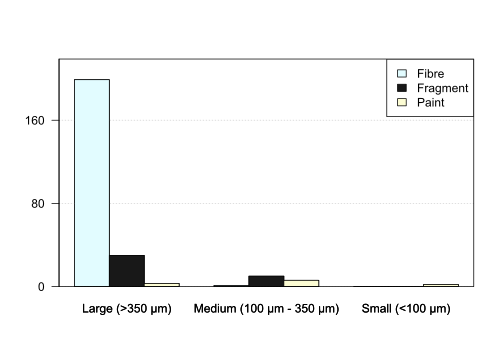
\includegraphics{mp-protocol_files/figure-latex/pieSize-1.pdf}
\caption{\label{fig:pieSize}Size distribution of the microplastic particles.}
\end{figure}

\hypertarget{colour}{%
\section{Colour}\label{colour}}

The most dominant colour was blue (64 particles) followed by transparent (57 particles) and black (56 particles). Color distribution, including less abundant colors, is shown in the graph below.

\begin{figure}
\centering
\includegraphics{mp-protocol_files/figure-latex/pieColour-1.pdf}
\caption{\label{fig:pieColour}Color distribution of the microplastic particles.}
\end{figure}

\hypertarget{particles-per-sampling-trip}{%
\section{Particles per sampling trip}\label{particles-per-sampling-trip}}

Sampling was carried out between April and October 2019 (total of 63 samples). Three samples were taken during each sampling trip (21 sampling trips). The average and standard deviation was calculated from each sampling trip and is shown in the graph below.

Numbers of particles are very low which could be attributed to the analytical method (stereoscopic observation) which only allows us to detect bigger particles (see graph above).

Mean particle abundance per sample ID was 1.2 (± 2.3).

As shown in the graph the standard deviation is very high which means there is big variability between the three samples. To improve this more samples could be taken. Another idea could be to sample a bigger volume of water to increase the number of particles. Instead of using a stereo microscope to detect the particles a more sensitive method could be used to be able to detect smaller particles and thus improve variability.

Blanks during sampling were taken from July onwards and are represented as black bars in the barchart below. Number of particles in the blanks can be close to the number of particles found in the samples which makes it difficult to conclude on the real number of particle present in the samples.

\begin{verbatim}
## [1] 4.475241
\end{verbatim}

\begin{verbatim}
## Warning in arrows(barCenters, as.matrix(Mean - SD) * 1, barCenters,
## as.matrix(Mean + : zero-length arrow is of indeterminate angle and so skipped

## Warning in arrows(barCenters, as.matrix(Mean - SD) * 1, barCenters,
## as.matrix(Mean + : zero-length arrow is of indeterminate angle and so skipped

## Warning in arrows(barCenters, as.matrix(Mean - SD) * 1, barCenters,
## as.matrix(Mean + : zero-length arrow is of indeterminate angle and so skipped

## Warning in arrows(barCenters, as.matrix(Mean - SD) * 1, barCenters,
## as.matrix(Mean + : zero-length arrow is of indeterminate angle and so skipped
\end{verbatim}

\begin{figure}
\centering
\includegraphics{mp-protocol_files/figure-latex/barchartSD-1.pdf}
\caption{\label{fig:barchartSD}Number of microplastic particles per sampling trip.}
\end{figure}

\hypertarget{particles-per-cubic-meter-per-sampling-week}{%
\section{Particles per cubic meter per sampling week}\label{particles-per-cubic-meter-per-sampling-week}}

From the number of particles found per sampling trip the number of particles per cubic meter was calculated and is shown in the graph
As described above, the number of particles per cubic meters is very low with a mean of 0.9 (± 0.7) particles per cubic meter.

\begin{verbatim}
## Warning in arrows(barCenters, as.matrix(Mean - SD) * 1, barCenters,
## as.matrix(Mean + : zero-length arrow is of indeterminate angle and so skipped
\end{verbatim}

\begin{figure}
\centering
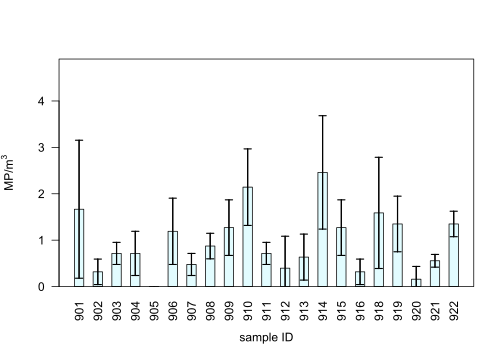
\includegraphics{mp-protocol_files/figure-latex/m3-1.pdf}
\caption{\label{fig:m3}Microplastic particles per cubic meter per sampling trip}
\end{figure}

\hypertarget{summary}{%
\section{Summary}\label{summary}}

In theory particle number should increase with decreasing particle size but that is not the case when analysing the samples with a stereo microscope.

Since the mean particle number was around 1.3 (± 2.3) per sampling trip and the mean number of particles found in the blank was around 0.5 (± 1.3) per sampling trip our findings are not very meaningful.

The number of detected MP particles must be well above blank samples!!!

\hypertarget{improvementsideas}{%
\section{Improvements/Ideas}\label{improvementsideas}}

\begin{enumerate}
\def\labelenumi{\arabic{enumi}.}
\tightlist
\item
  Start finding a purpose of the monitoring programme, and set its aims!
\end{enumerate}

\begin{itemize}
\tightlist
\item
  If the purpose of the monitoring is to detect long-term trends, of microplastics in the marine environment, sediments might be the most suitable matrix since it is the sink where most particles will be sequestered (collect where MPs are likely to accumulate)
\item
  If the purpose of the monitoring instead is to detect time trends of microplastic emissions from a point source, such as a wastewater treatment plant or an industry, sampling of the water surface or water column would ideally provide information on the single process or pathway.
\end{itemize}

\begin{enumerate}
\def\labelenumi{\arabic{enumi}.}
\setcounter{enumi}{1}
\tightlist
\item
  We need to change our sampling in order to increase the number of particles in each sample (e.g.~by increasing sampling volume and decreasing mesh size or measuring smaller particles with the same mesh size, \ldots).
\end{enumerate}

\begin{itemize}
\tightlist
\item
  „Regardless of which method is applied, most important is to ensure that the samples contain a high enough number of particles and to take enough replicates to allow for statistical analysis of data. This is vital in order to compensate for uncertainty related to counting statistics and patchiness of microplastic particles within the confined sampled space (Karsson et al.~2018).``
\end{itemize}

\begin{enumerate}
\def\labelenumi{\arabic{enumi}.}
\setcounter{enumi}{2}
\item
  Try to avoid sand in our samples to eliminate the density separation step (avoid sampling to close to the sea bed)
\item
  Our filters still seem to contain a lot of chitinous zooplankton carapaces after our digestion protocol with KOH and H2O2
\end{enumerate}

\begin{itemize}
\tightlist
\item
  Try to digest with chitinase enzymes
\item
  Another idea would be to use the Raman to check the chemical composition of the organic matter which is left on the filters to improve the digestion method (then we would be able to specifically target certain polymers like chitin, cellulose,.. and digest them accordingly).
\end{itemize}

\begin{enumerate}
\def\labelenumi{\arabic{enumi}.}
\setcounter{enumi}{4}
\item
  Organic material needs to be digested further on our samples if automated spectroscopic analysis with Raman will be applied
\item
  In addition to internal blanks, recoveries of reference particles in different size fractions and external QA procedures should be included
\end{enumerate}

\hypertarget{other-notes}{%
\section{Other notes:}\label{other-notes}}

\begin{itemize}
\tightlist
\item
  The abundance of microplastics, as for most other particles, increases exponentially with smaller sizes, and therefore all recent environmental risk assessment reports emphasize the role of smaller MP sizes
\item
  Studies show that data from surface water only (like with manta net) does not provide a complete picture of the amount of microplastics in water.
\item
  It should be emphasized that both the visual analyses with stereomicroscopy (to reveal the particle shape, colour and texture) and the interpretation of spectra from FTIR and Raman spectroscopy (to identify the polymer composition of the particles) require a well-trained staff if the results are to be reliable.
\item
  The more digestion steps are applied the higher the risk of contamination and the higher the risk of loss of particles in the samples
\item
  When using ZnCl2: precipitation can form with high alkaline solutions (ZnOH2)
\item
  ZnCl2: a larger number of non-plastic particles will float up to the surface, making the analysis of samples more difficult
\item
  When working with ZnCl2: it is classified as toxic to humans and hazardous to the aquatic environment, and all the liquids and sediment need to be treated as chemical waste!!!
\item
  The depth where water samples are being collected, or the sampling season can make a crucial difference in the amounts and types of organic material present in the samples -\textgreater{} affecting the selection of most suitable digestion methods.
\item
  The requirements for sample quality and purity are higher when aiming to analyze smaller particles
\end{itemize}

\hypertarget{sampling-and-processing-dates-of-2019}{%
\chapter{Sampling and processing dates of 2019}\label{sampling-and-processing-dates-of-2019}}

\includegraphics{mp-protocol_files/figure-latex/SamplingProcessingDates-1.pdf}

\hypertarget{efficiency-of-digestion}{%
\section{Efficiency of digestion}\label{efficiency-of-digestion}}

Samples 901-906 could not be weighed as those samples were put onto a GF/C filter which seems to have lost weight after filtration. Hence samples 901-906 could not give us information about the digestion efficiency.
Samples 907-909 were put onto a membrane filter (0.22 um) and samples 910-922 were put onto the normal Nitrocellulose filters. Weight was taken from all filters after they had been dried at room temperature for several weeks.
The median digestion efficiency was 92 \% which means that 92 \% of the organic matter present in the beginning was digested. The average digestion efficiency was at 88 \%.
The amount left behind on the filter after digestion correlates with the amount of organic matter originally present in the samples.
Digestion efficiency was below the average in samples 915, 916, 917, 918 and 920. Possibly because of high content of diatoms.

\includegraphics{mp-protocol_files/figure-latex/DigestionEfficiency-1.pdf}

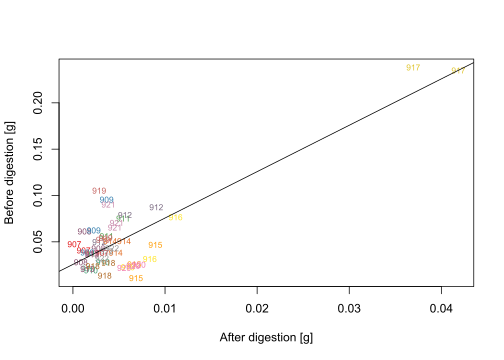
\includegraphics[width=0.5\linewidth]{mp-protocol_files/figure-latex/MyndDigestionEff-1} \includegraphics[width=0.5\linewidth]{mp-protocol_files/figure-latex/MyndDigestionEff-2}

  \bibliography{refs.bib}

\end{document}
